\section{Memory-Related Performance Problems}\label{sec:background}
As modern computing systems evolve, the demand for increased computational power and memory resources has become more prevalent. This demand is driven by the increasing complexity of applications and the need to process larger amounts of data. In this section, we will explore the challenges and performance problems that from the ever-growing requirements for memory and computational resources. We begin by discussing the processor-memory speed gap and its implications (\ref{sec:pmgap}), followed by a brief examination of the increasing computational and memory requirements of modern applications (\ref{sec:comp_mem_req}). The processor-memory speed gap and the increasing computational and memory requirements combined result in a need to tackle high data transfer costs and bottlenecks (\ref{sec:data_transfer}). Finally, as a solution to the aforementioned problems, we will define the concept of data locality (\ref{sec:data_locality}).

\subsection{Processor-Memory Performance Gap}\label{sec:pmgap}
It is well known, that the performance of CPU's doubles roughly every two years, a phenomenon resulting from Moore's law. Similarly, memory technology has also been improving at an exponential rate, however at a slower rate \cite{efnusheva2017survey, machanick2002approaches, mckee2004reflections, mccalpin1997survey}. Since the difference between two exponential functions is also exponential, this gap will also increase at an exponential rate. This is known as the processor-memory performance gap. Figure \ref{fig:pmgap} illustrates this trend in improvements in computational and memory performance, measured by floating point operations and memory operations per second, respectively.

\begin{figure*}
	\begin{subfigure}{.5\textwidth}
		\centering
		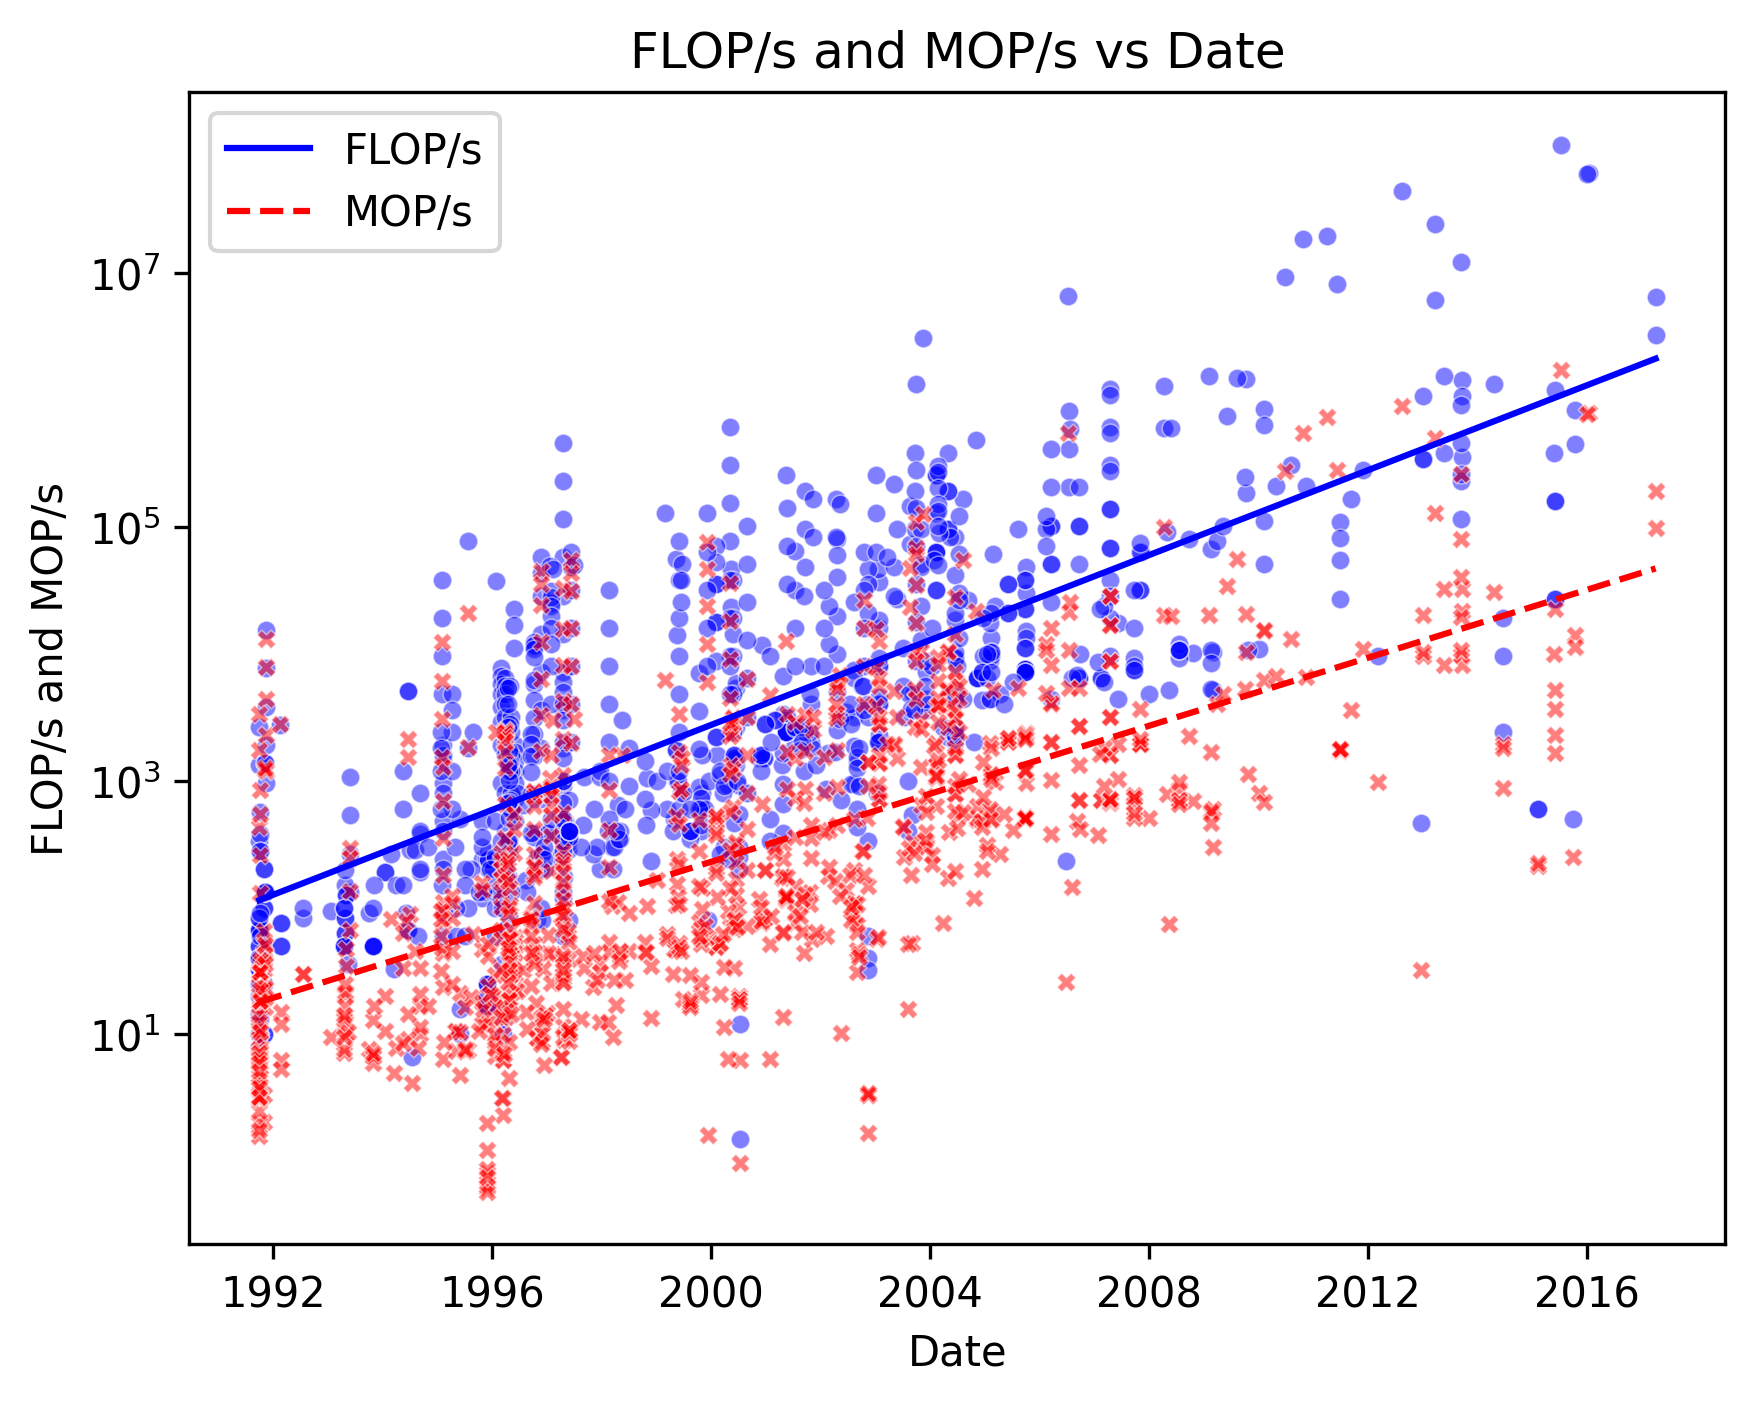
\includegraphics[width=.9\linewidth]{pictures/FLOPs_MOPs_vs_Date.png}
	\end{subfigure}
	\begin{subfigure}{.5\textwidth}
		\centering
		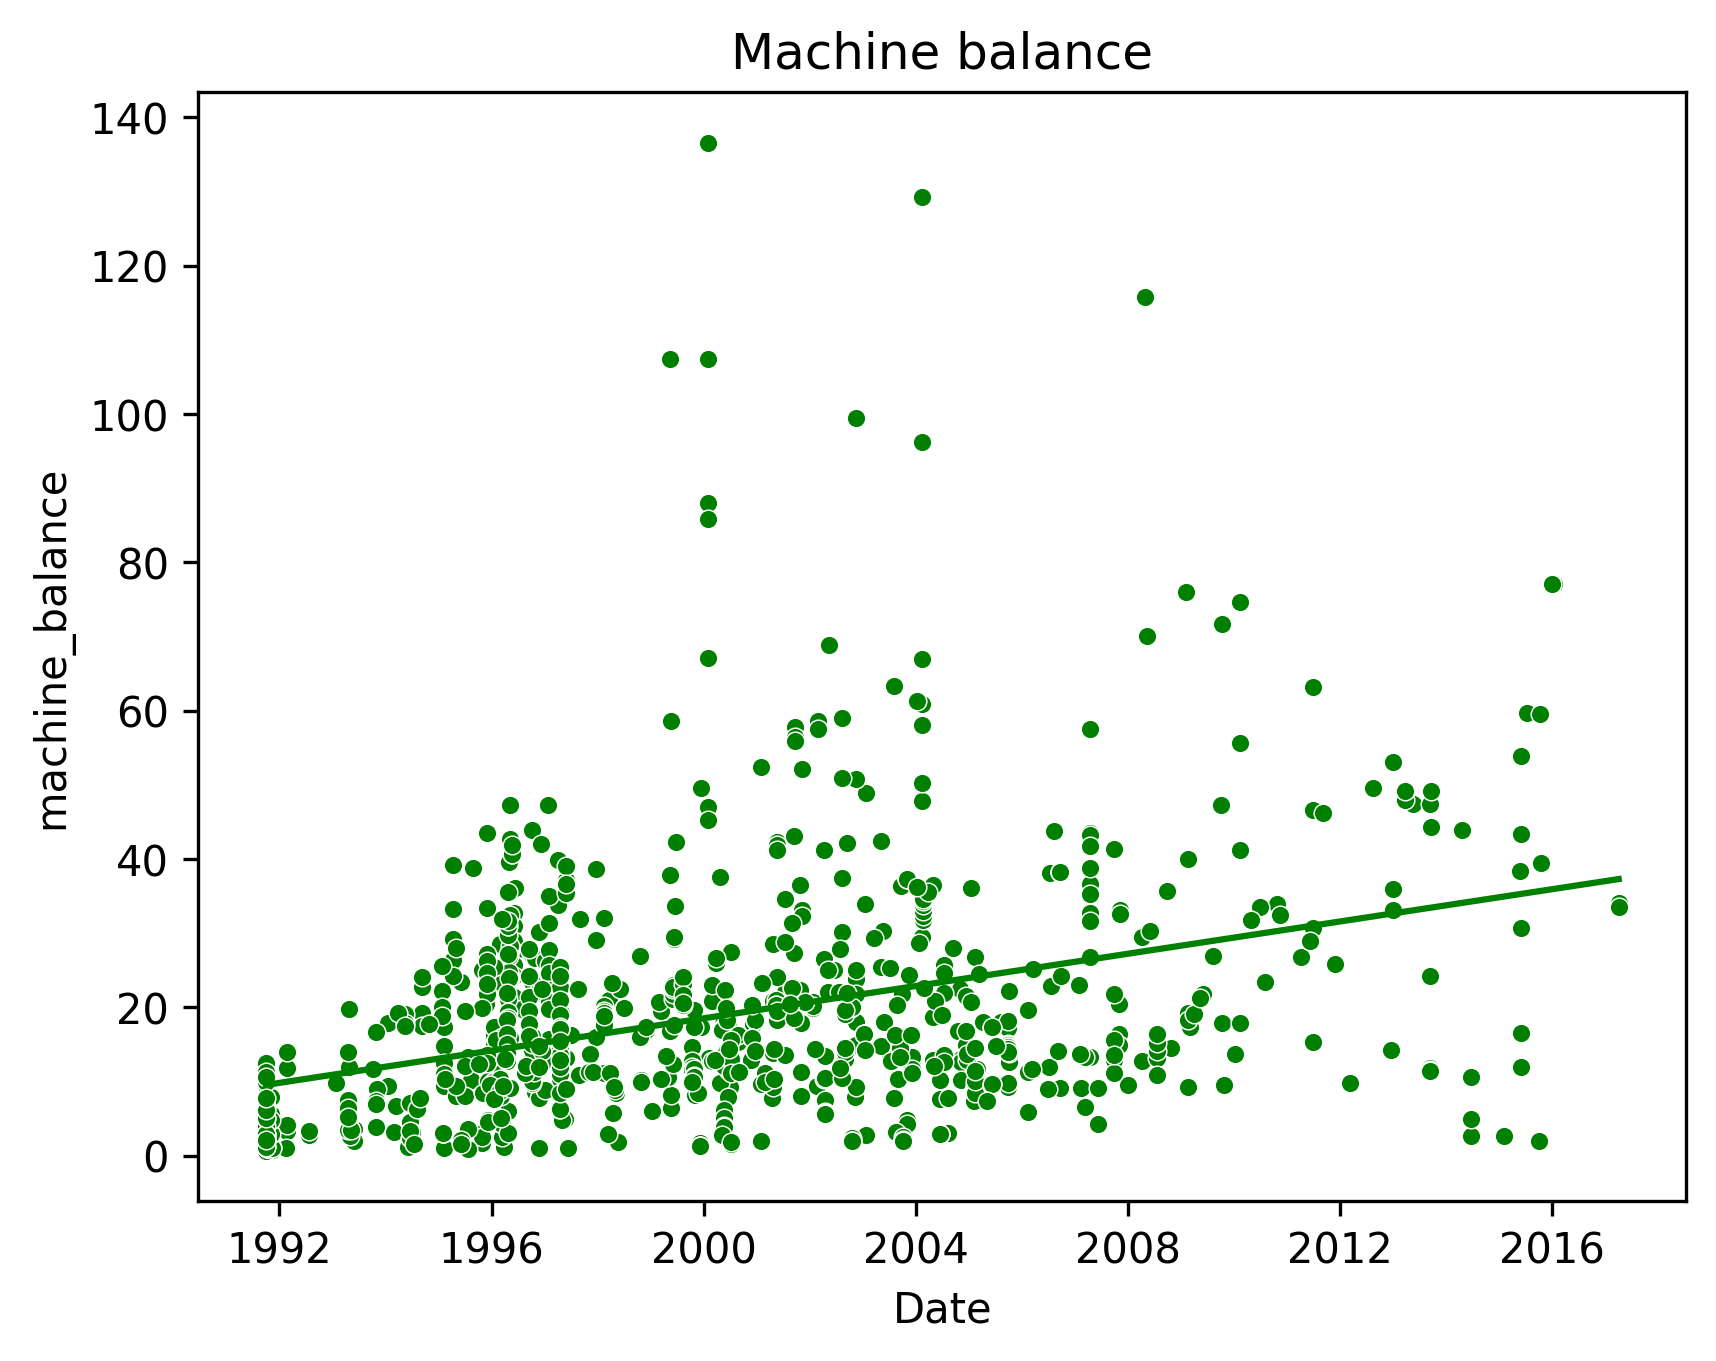
\includegraphics[width=.9\linewidth]{pictures/machine_balance.png}
	\end{subfigure}
	\caption{Illustration of the expanding Processor-Memory Gap. The left graph charts the progression of FLOPs and MOPs on a logarithmic scale across various computing platforms, with the FLOPs trendline demonstrating a steeper ascent, indicative of the widening gap. The right figure depicts the development of the machine balance score for these platforms.\protect\footnotemark{}}
	\label{fig:pmgap}
\end{figure*}
\footnotetext{Data was acquired from a collection of STREAM benchmark results on \url{https://www.cs.virginia.edu/stream/}.}

The increasing processor-memory performance gap becomes a critical problem, when considering data access times. Let us take the equation for the average memory access time:
\begin{equation}\label{eq:avg_mem_time}
t_{avg} = p \cdot t_c + (1-p) \cdot t_m
\end{equation}
Here, $p \in \left[0,1\right)$ denotes the probability of a cache hit. As at least one instruction has to be fetched from the memory, at least one cache miss is guaranteed, thus $p < 1$. $t_c$ and $t_m$ denote the times to access data from a cache and the main memory, respectively \cite{wulf1995hitting, mahapatra1999processor}. Without loss of generality, let us consider these times in terms of number of clock cycles.

As a result of the increasing processor-memory performance gap, $t_m$ (and to a lesser extent $t_c$) will be increasing exponentially, taking more and more clock cycles to access the same amount of data - clock cycles that could be used to perform calculations. As a result, the overall system performance will be increasingly determined by memory performance. At some point, CPU's will be able to execute code faster than we can feed them with instructions and data. For this reason, the processor-memory performance gap is also known as the memory wall problem \cite{wulf1995hitting, mckee2004reflections, mahapatra1999processor}.

The notion of Machine Balance has been introduced, which quantifies the processor-memory performance gap \cite{mccalpin1997survey, mccalpin2016memory}:
\begin{equation}\label{eq:machine_balance}
	balance = \frac{peak\; FLOP/s}{sustained\; MOP/s}
\end{equation}
This metric, also depicted in Figure \ref{fig:pmgap}, is a measure of how well a system is balanced between computational and memory performance. A balance of 1 indicates a perfectly balanced system, whereas $balance \ll 1$ or $balance \gg 1$  indicates a system that is completely compute bound or completely memory bound, respectively \cite{mccalpin1997survey, mccalpin2016memory}.

\subsection{Computation and Memory Requirements}\label{sec:comp_mem_req}
Different applications have different requirements for system resources. There exist some programs that have a larger computational demand, thus benefiting from a higher machine balance (section \ref{sec:pmgap}) \cite{mccalpin2016memory}. However, the memory wall problem states that it will be increasingly more difficult for such applications to exploit further advances in computational performance, as for any application the memory performance will grow to be the limiting factor \cite{wulf1995hitting, mckee2004reflections}.

Furthermore, we notice that computational as well as memory requirements are increasing rapidly. A prime example of this is the field of artificial intelligence systems, which currently sees an exponential growth in the number of parameters used \cite{ourworldindata2023ai}. Hence, for any application, regardless of its computational or memory demands, it is crucial that significant strides are made in enhancing both the processing and memory capabilities. This ensures that the constraints imposed by the memory wall problem do not inhibit the potential performance of these applications.

\subsection{Data Transfer Costs and Bottlenecks}\label{sec:data_transfer}
\paragraph*{Memory Latency} Memory latency, as discussed in section \ref{sec:pmgap}, pertains to the time delay between a request to access data from the main memory and the actual execution of this operation. Increasing memory latencies, measured in terms of clock cycles, lead to the processor waiting longer for data, which significantly tightens the performance bottleneck. This latency challenge can adversely impact the execution of applications, and its reduction is often a complex task \cite{machanick2002approaches}.
\paragraph*{Memory Bandwidth} Memory bandwidth is a measure of the volume of data that can be transferred to or from the memory per unit time. A bottleneck arises when the bandwidth is insufficient to handle the required data transfer volume, causing the processor to wait for data \cite{machanick2002approaches}.
\paragraph*{Cache Misses} Multi-level memory hierarchies were introduced to hide memory latencies. Here, faster, but also more costly and thus smaller memory modules are being placed between the CPU and the main memory. These are referred to as caches. When a processor requests data from the memory, it first checks if the data was already preloaded into the cache. If so, the data can directly be loaded from the cache - a cache hit has occurred. However, if the data is not present in the cache, it has to be fetched from the main memory, which, due to its higher latency, takes significantly longer. This is referred to as a cache miss \cite{efnusheva2017survey, mahapatra1999processor, machanick2002approaches}. As the loading of data into caches occurs through software, poor cache management can lead to a significant performance degradation.

\subsection{Data Locality}\label{sec:data_locality}
Data locality is a key concept in enhancing memory performance and therefore mitigating the implications of the processor-memory performance gap. It refers to the tendency of a processor to access the same set of memory locations repetitively over a short period of time. This concept capitalizes on the multi-level memory hierarchy of modern computers. By improving data locality, one reduces the number of cache misses (section \ref{sec:data_transfer}), or equivalently, reduces $p$ in equation \ref{eq:avg_mem_time}, improving overall system performance \cite{unat2017trends, tate2014programming}.

There are two main types of data locality: temporal and spatial. Temporal locality refers to the reuse of specific data, within a relatively small duration. This means that if a memory location is accessed, it is likely that the same location will be accessed again in the near future. Spatial locality, on the other hand, refers to the use of data items within relatively close storage locations. In other words, if a memory location is accessed, it is likely that memory locations nearby will be accessed soon \cite{esseghir1993improving}.

Data layout plays a significant role in the realization of data locality, as it can substantially influence the memory access patterns and hence, the performance of a program. A thoughtful arrangement of data in memory can encourage both temporal and spatial locality, thus reducing cache misses and enhancing the overall system performance \cite{esseghir1993improving}.

To illustrate, consider a two-dimensional array laid out in memory, where elements in the same row are placed in contiguous memory locations. Now let an application iterate through this array in a row-major order. Because of the memory layout, it benefits from spatial locality as accessing one element in a row makes it likely that the next element will be accessed soon, thus reducing the number of cache misses. On the contrary, if the application were to traverse the array in a column-major order, it would not benefit from spatial locality due to the dispersed memory locations of elements in the same column, leading to a higher rate of cache misses and reduced performance.

While this example demonstrates a simple scenario, the reality is often more complex, especially for larger and more intricate applications. Understanding the data access patterns of an application is key to deciding the best data layout, and this often requires an intimate knowledge of the program's structure. Moreover, optimizing data locality can be quite challenging due to the diversity of hardware architectures. The same program can exhibit different data locality characteristics on different hardware due to variations in the memory hierarchy (such as cache sizes and levels, memory bandwidth, and latency).

This paper will provide an overview of an approach to optimize data locality with the help of visualizations.
